%-------------------------------------------------------
%    DOCUMENT CONFIGURATIONS
%-------------------------------------------------------

%-------------------------------------------------------
%    START OF COMMUNICATION ANALYSE
%-------------------------------------------------------
\subsection{Communication}
\label{sub:communication}
Considered to be the most important of the project, without internodes communication, Overclouds has no meaning. We are also aiming at a browser only system, leading into looking at modern technologies written in Web-driven languages.

\paragraph{Propagation} We started to look at homemade solutions. In the cases of communication by data propagation, the path optimization will not be possible, and the global status of the network will be tough to maintain. Plus, it will not be easy to be sure that the chunk arrived at the destination. However, it is easy to push data into the void. Also, note, that a protocol must be made to avoid to the propagation of the source address and preserve anonymity.

\paragraph{3rd parties} The most common way to do peer-to-peer from the browser is to relay on a 3rd party service to do the signaling and put peers into relation. To preserve the anonymity and security integrity, we must, in this case, maintain a list of \textit{trusted} nodes (gateways) by the consensus to join the network. We could use TOR technology, Figure ~\ref{fig:tor-scheme} in the annexes, but a browser only integration is not done yet. The 3rd party services could be either servers running custom code, for example, wrote in NodeJS, either companies specialized into signaling services like peer5\cite{Peer52015Peer5}, openpeer\cite{Hookflash2014OpenPeer}, peerjs\cite{SwitchPeerJS}, etc. In the second case, we must give even more trust into their services (hosting and signaling), we are hardly favorable on this option, how can we ensure their services will not be shut down or will not censor our project because they do not like it or if they are asked to do so?

\paragraph{Organization's Server} If the 3rd party servers solution is selected. It could be interesting to create a protocol that gives the consensus the control over the servers and manage the costs. Indeed, a consensus-driven payment via crypto-currencies directly to the 3rd party host could be interesting, but it would mean that the consensus owns capitalized crypto-currencies. We could imagine that the network would mine crypto-currencies.

\subsubsection{WebRTC}
Pushed by HTML5 standards and companies like Google, Mozilla, Opera, etc. WebRTC\cite{GoogleWebRTC} provides a clear API, optimized for Real-Time Communications (RTC), in an always growing developer community, and the major browsers supported (Chrome, Firefox, and Opera). Note the Chrome and Firefox have interoperability. However, a server is needed for the signaling (sort of tracker).

\paragraph{Datachannel\cite{R.Stewart2007StreamProtocol}} Based on top of the basic WebRTC, and almost real-time,  the main limitation is peers' speed connection and Javascript itself. It has two modes, \textbf{reliable mode}, which provides TCP-like guaranteed packets' order and no loss. Moreover, the \textbf{unreliable mode} which provides like UDP no guarantees for the data transfer. It allows encrypted communication and data transfer between compatible browsers (Chrome and Firefox). However, a threat still exists, it is people. Indeed, that can send malicious data like a virus to other peers. Note that the transfer is said to be secure at the moment, but it is not infallible, it is recommended to encrypted the data before the transfer. In Overclouds, we would encrypt each chunk. Like the basic WebRTC, linking peers is done by signaling servers.
The figure ~\ref{fig:signaling-advanced} schematize an advanced procedure to make a data channel between two clients, which should prevent censorship or freaky firewalls.
\begin{figure}[htpb]
\centering
\caption{\small \sl Advanced Data Channel
\label{fig:signaling-advanced}}
\begin{adjustbox}{center}
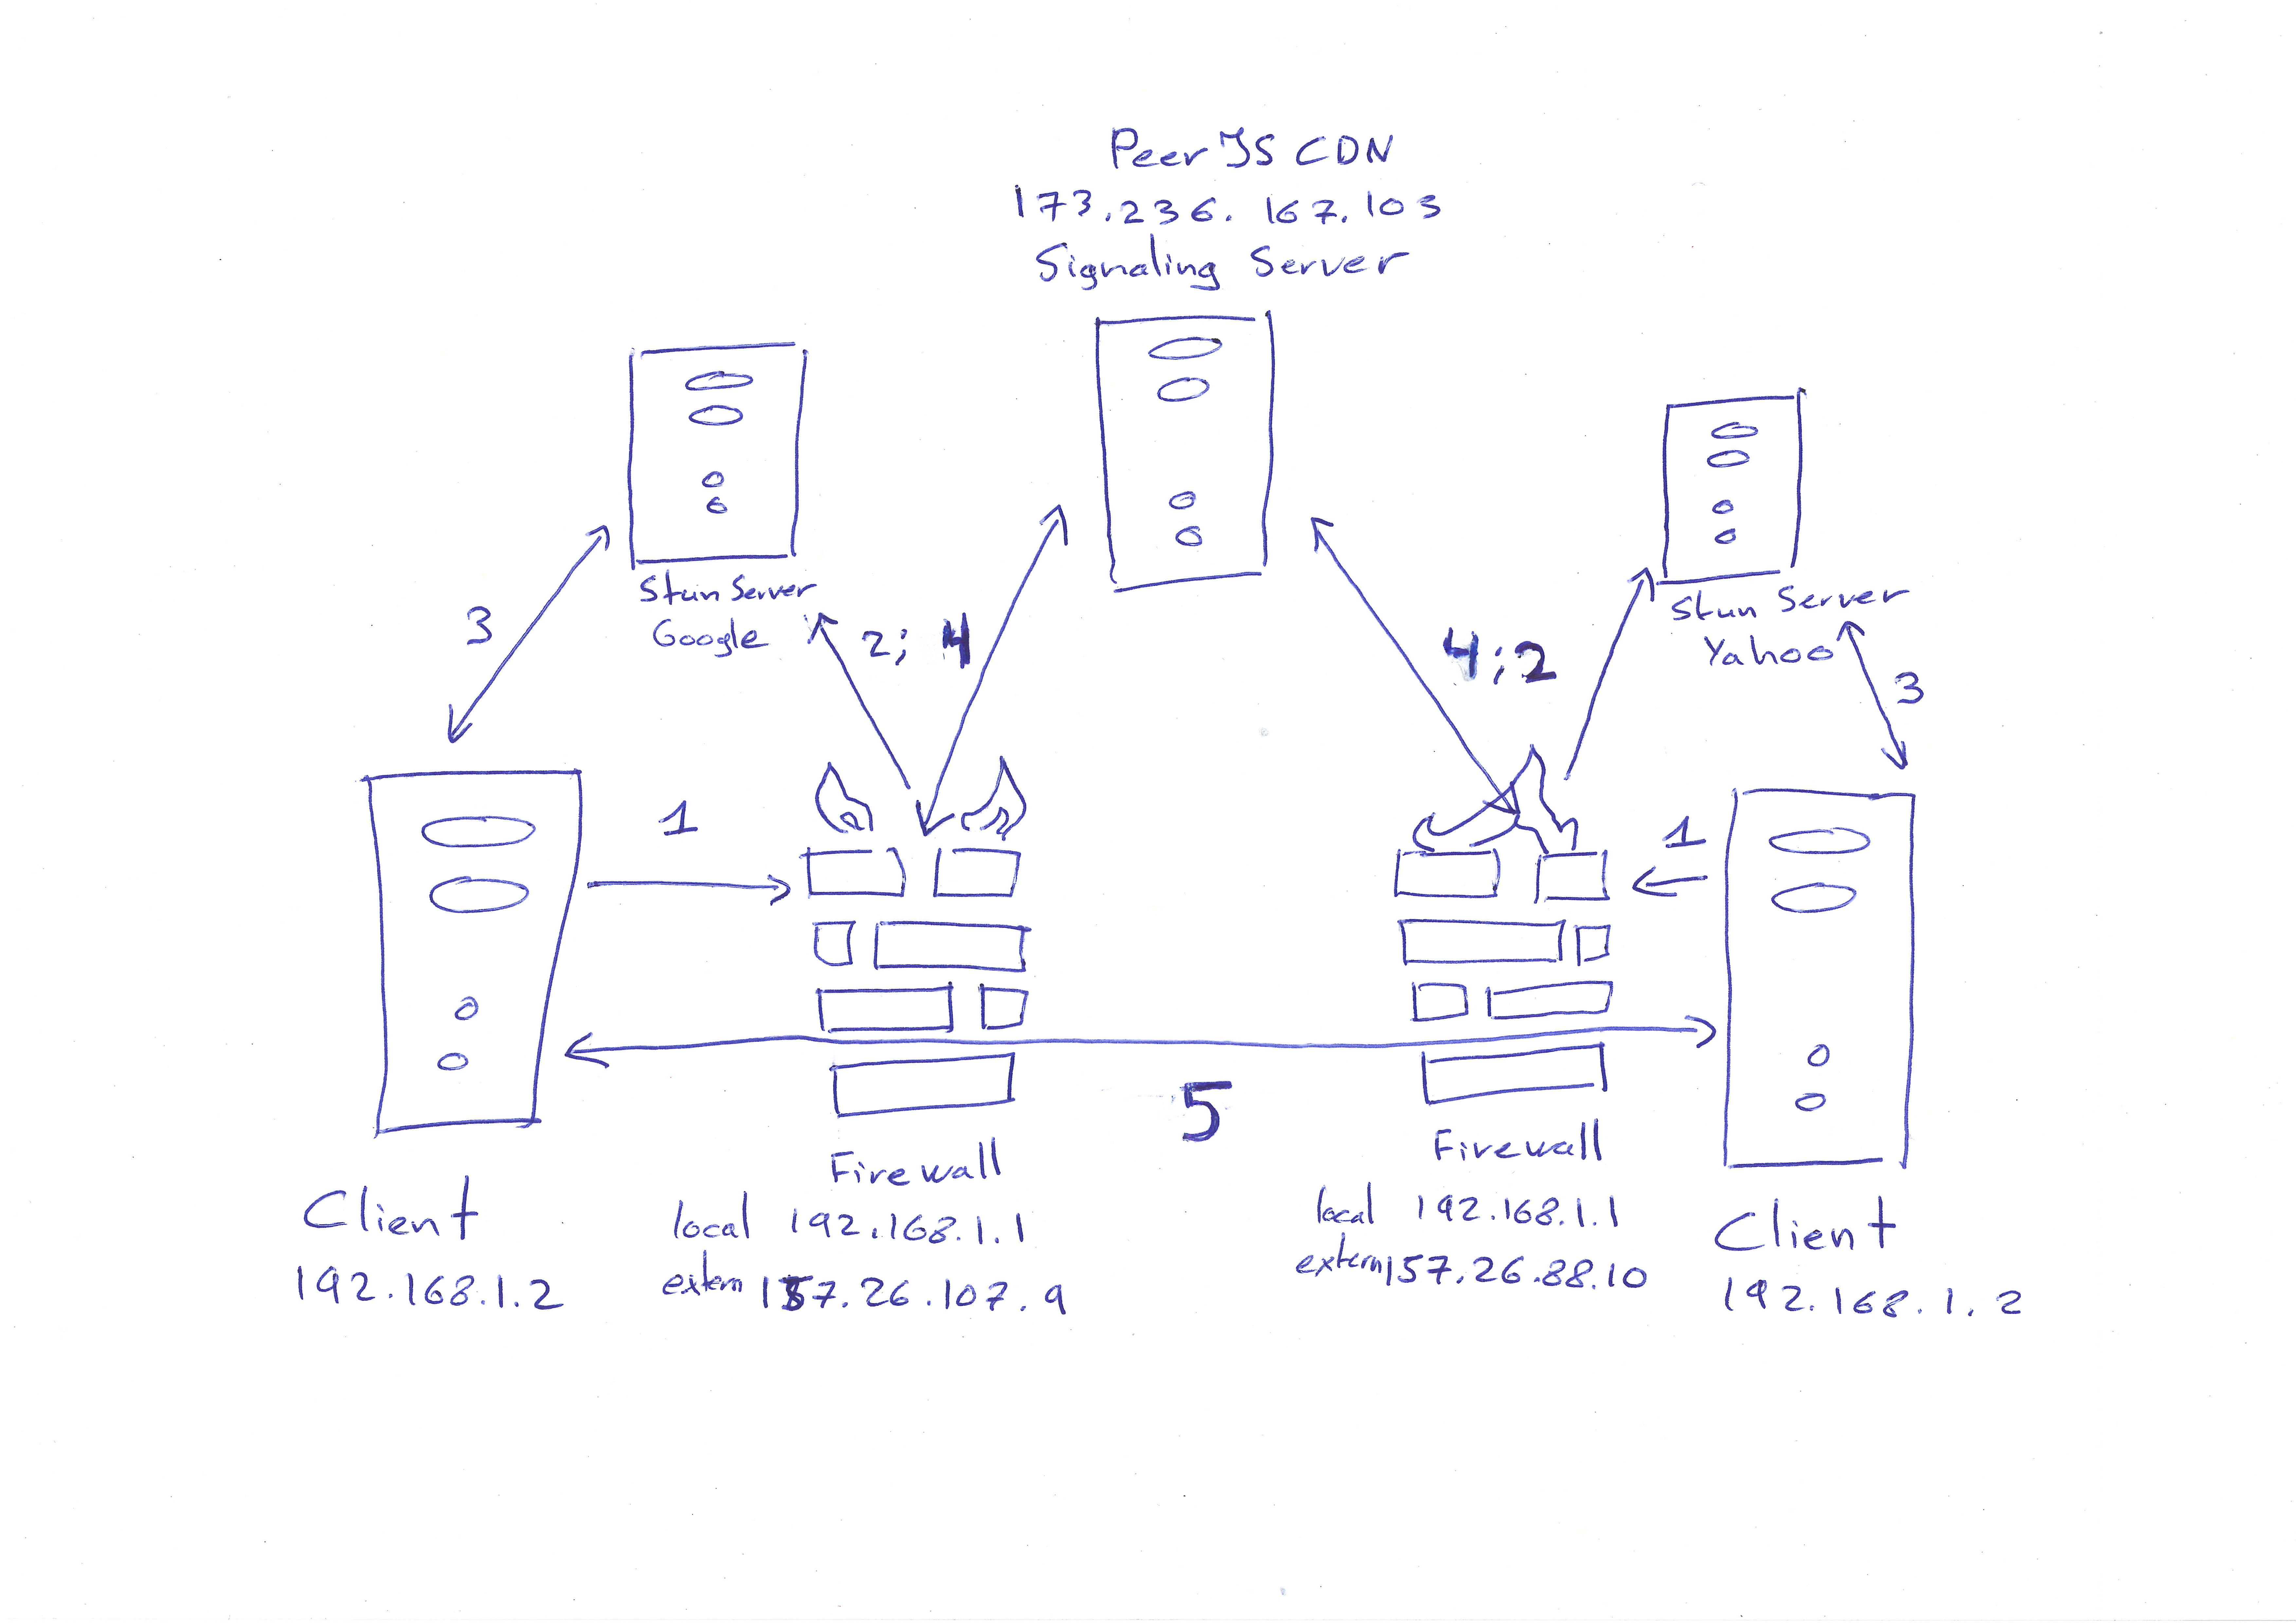
\includegraphics[scale=0.1]{annexes/schemes/signaling-advanced.jpg}
\end{adjustbox}
\end{figure} 
\clearpage

\subparagraph{ORTC} On the other end, Object real-time communications technology is pushed by W3C \& Microsoft. It is younger than WebRTC, 2011 vs. 2014, the main difference\cite{Sinch2015ORTCDIFFERENCE} between the two protocols is the supported media protocols and also the fact that ORTC does not have a standard for its signaling protocol. It is not clear today, what major differences will be between them in the future.

\subsubsection{Overclouds}
\label{subsec:overclouds}
By taking the pros and the cons of the previous communication solutions. Our choice goes to \textbf{WebRTC Datachannel} is the close technology to our needs. However, the signaling requirement was challenging. The solutions would be to have a trusted signaling node list controlled by the consensus. 

\paragraph{Serverless} The main problem we were confronted with while doing research on WebRTC, was the incompatibility with Overclouds' vision of browser only need, read as the user should not install any software expect a browser to be able to connect to the network. We finally found a solution to use the very promising WebRTC, however, the downside is the signaling procedure, which centralizes the tracking of nodes on the network, but it could be accepted if the server is trusted and maintained by the consensus. To our greatest pleasure, during the implementation, we found a solution to make the signaling procedure serverless. Users will still need to communicate their secret peer address somehow, but the addresses will not be managed via a 3rd party. The next step will be to find a procedure to transmit the peer address securely.
The figure ~\ref{fig:stun-scheme} schematize how the hole is made in the firewall with STUN servers.
\begin{figure}[htpb]
\centering
\caption{\small \sl Serverless STUN Scheme
\label{fig:stun-scheme}}
\begin{adjustbox}{center}
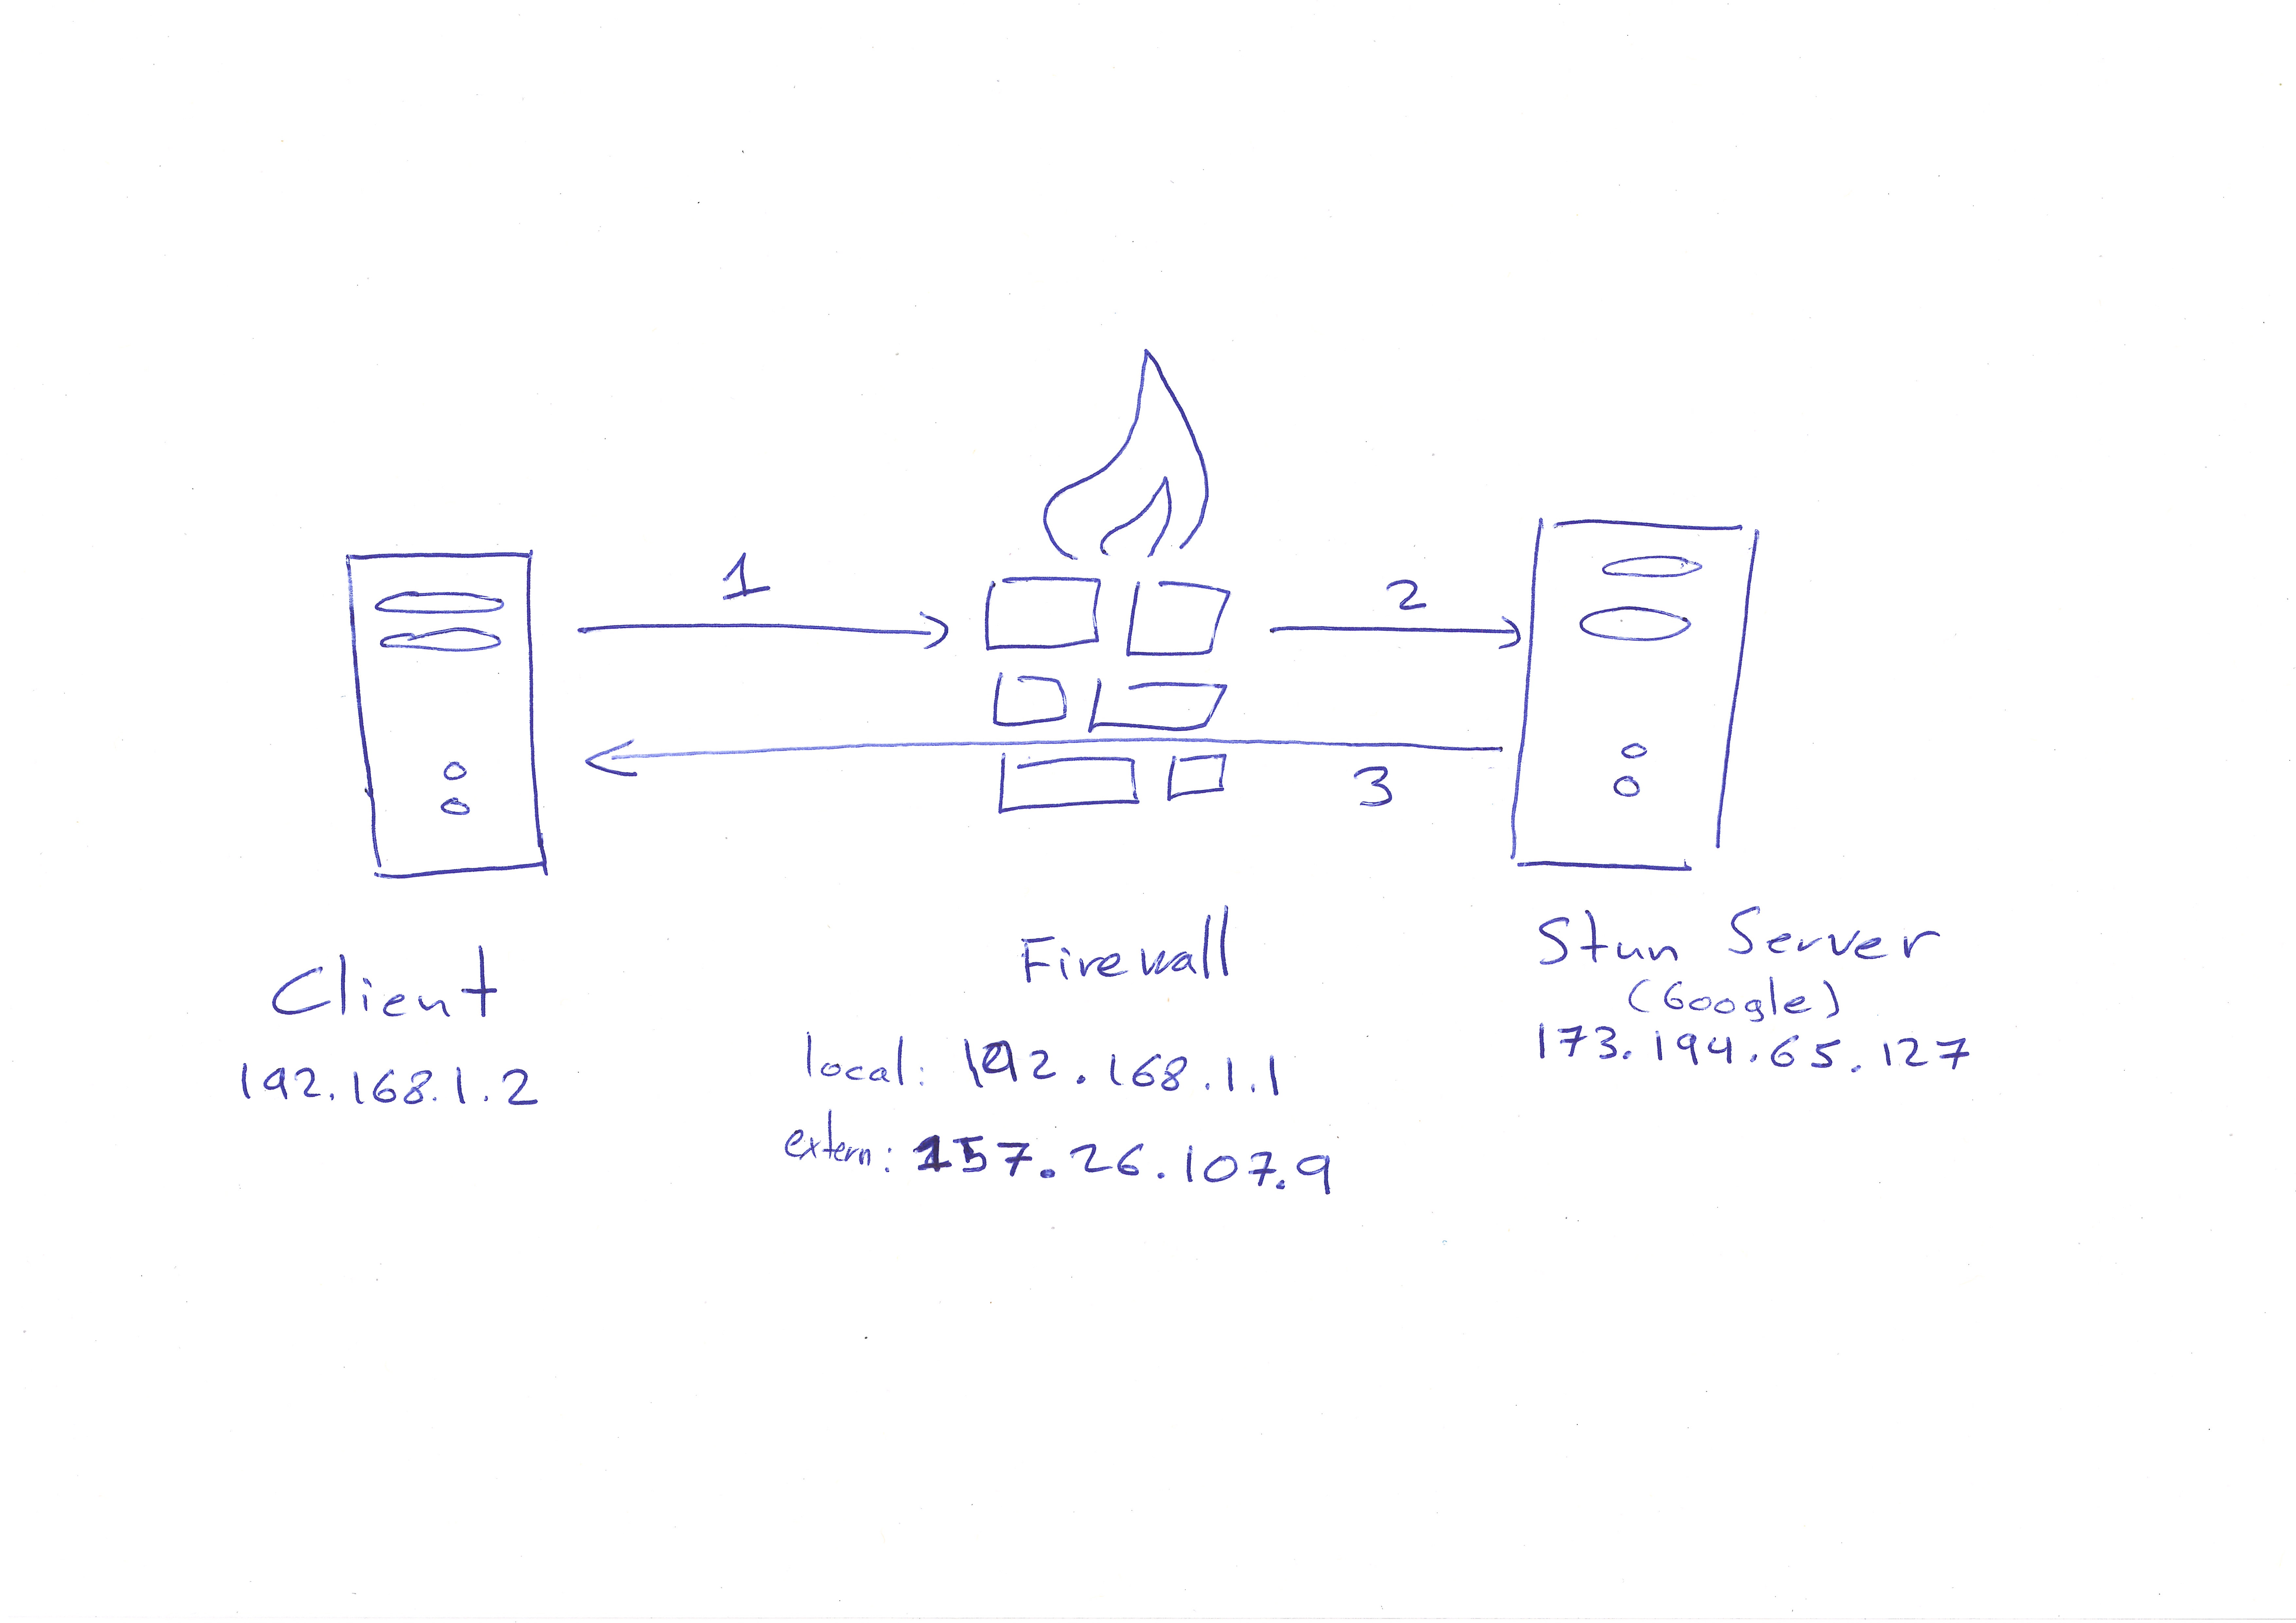
\includegraphics[scale=0.1]{annexes/schemes/stun-scheme.jpg}
\end{adjustbox}
\end{figure} 

%-------------------------------------------------------
%    END OF COMMUNICATION ANALYSE
%-------------------------------------------------------